\chapter{Internet of Threads}                %crea il capitolo
%%%%%%%%%%%%%%%%%%%%%%%%%%%%%%%%%%%%%%%%%imposta l'intestazione di pagina
\lhead[\fancyplain{}{\bfseries\thepage}]{\fancyplain{}{\bfseries\rightmark}}
\pagenumbering{arabic}                  %mette i numeri arabi
\section{Definizione}                 %crea la sezione
L'internet of things, ovvero l'internet delle cose, vuole rappresentare la diffusione dei sistemi embedded come veri e propri nodi di reti. Nell'ottica dell'IoT, oggi, apparecchi comununi in un'abitazione, quali condizionatore, la caldaia o addirittura il tostapane, possono essere nodi di rete ed essere quindi configurati e controllati attraverso di essa.\\
Il concetto di internet of threads \`e una evoluzione di questa astrazione. L'idea alla base di IoTh \`e quella di avere non solo oggetti ma anche processi come nodi di rete.\\
Per poter capire pienamente i vantaggi dell'IoTh si pu\`o pensare ad un'analogia con quanto \`e successo nel mondo della telefonia. In passato la telefonia collegava apparecchi fissi collegati via cavo, in questo modello il numero di telefono individuava un luogo e non una persona e quindi era comunque, per trovare una persona, doversi interrogare sul dove questa potesse essere; al contrario l'avvento dei telefoni cellulari ha cambiato l'idea di significato di numero di telefono, non pi\`u associato a luoghi fisici ma ad una persona infatti i telefoni cellulari sono normalmente telefoni personali\cite{K1,K2}.\\
Come possiamo notare infatti, con questa tecnologia lo stack \`e direttamente integrato nel programma.
\begin{figure}[h]
\centering
\begin{minipage}{.5\textwidth}
\centering
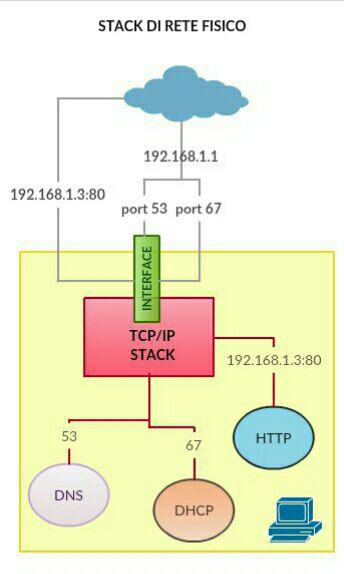
\includegraphics[width=7cm]{old_stack}
\caption[physical interface stack]{stack associato\\ all'interfaccia fisica}\label{fig:fisical}
\end{minipage}%
\begin{minipage}{.5\textwidth}
\centering
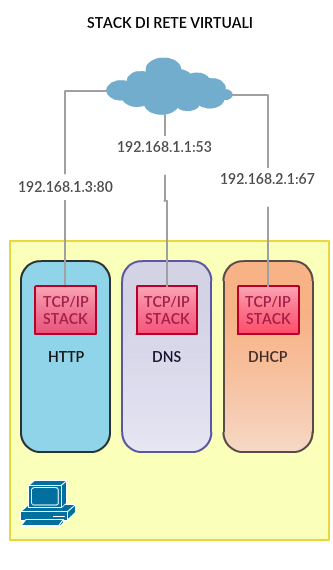
\includegraphics[width=7cm]{new_stack}
\caption[virtual stack]{stack associato\\ ai processi}\label{fig:virtual}
\end{minipage}
\end{figure}\\
Nello stesso modo IoTh indirizza i processi che forniscono un servizio, questo significa che questi processi non sono pi\`u vincolati a risiedere in un luogo specifico, in un elaboratore specifico nell'ambito delle reti, ma \`e possibile trasparentemente farli migrare da un elaboratore all'altro senza che questo crei difficolt\`a di indirizzamento.\\
Una nota va anche fatta in termini di sicurezza. La possibilit\`a che ogni servizio utilizzi propri indirizzi IP e uno stack di rete privato rende molto pi\`u difficile se non praticamente impossibile sfruttare le fragilit\`a di un servizio per poter scalare l'intrusione ad altri servizi presenti sullo stesso sistema.

\section{Stack Implementati}
Diversi sono i progetti che si occupano di offrire ai processi il proprio stack di rete; tra questi ne verranno presi in esame tre, considerati pi\`u indicati per uno studio in quanto open source, Ognuno di essi offre la propria implementazione di stack di rete.\\
Uno stack di rete legato al processo permette di connettere lo stesso ad una rete reale, tramite le interfacce fornite dal sistema, o virtuale (ad esempio VDE) come se fosse una macchina fisica a se stante, a questo punto ogni processo pu\`o staccarsi dal modo in cui la macchina che lo ospita gestisce la rete ed avere le proprie regole.\\

\subsection{PicoTCP}
Supportato da Tass Belgium (Altran); \`e lo stack pi\`u conosciuto e diffuso per sistemi embedded ed esistono anche dei progetti basati su IP di reti mesh realizzati con picoTCP\footnote{http://www.picotcp.com/mesh-design-guide}.\\
Purtroppo per motivi commerciali alcune parti del codice non sono state rese pubbliche anche se rappresentano una piccola percentuale dell'intero progetto.
\subsection{LWIP}
Nasce come progetto di Adam Dunkels pensato per sistemi embedded ed inizialmente non forniva supporto ad IPv6.\\
Light-weight IP (LWIP) vanta un core molto piccolo e la possibilit\`a di eseguire anche senza sistema oprativo (single-threaded) e con il minor consumo di RAM possibile, inoltre \`e modulare ed offre la possibilit\`a di aggiungere protocolli come DHCP e DNS solo in caso di necessit\`a.\\
Supporta sia little che big endian e gira su processori a 8 e 32 bit, quindi funziona anche su un semplice ATMEGA.\\
Unica pecca \`e il protoccolo IPv6 che \`e ancora in fase sperimentale, infatti il supporto IPv6 pu\`o essere aggiunto ed \`e scaricabile da git.
\subsection{LWIPv6}
Precedemente si \`e notato che LWIP non aveva supporto IPv6 e che tutt'ora \`e ancora in fase sperimentale, ed \`e questo uno dei motivi della nascita di LWIPv6.\\
Quando al team di virtualsquare \`e sopravvenuta la necessit\`a di avere uno stack per la rete vde non esisteva ancora nulla di maturo o comunque plug and play, da questa esigenza il team ha pensato di realizzare uno stack versatile in versione libreria tale per cui ogni processo potesse avere il proprio stack di rete.\\
Caratteristica principale di LWIPv6 \`e il suo motore ibrido che, di fatto funziona solo con IPv6 e mappa in questo protocollo le comunicazioni IPv4 utilizzando i primi 80 bit dell'indirizzo come flag di riconoscimento con tutti e 80 impostati a 1, ad esempio se volessimo rappresentare la maschera 255.255.255.0, che in esadecimale \`e equivalente a 0xffffff00 e la sua rappresentazione in IPv6 secondo LWIPv6 sar\`a la seguente 0xfffffff.ffffffff.ffffFFFF.ffffff00.
\section{Netlink}
\subsection{Inter Process Communication}
Molti processi necessitano di scambiare informazioni per i motivi pi\`u disparati, dalla comunicazione di rete a quella interna ad una sola macchina.\\
Viene da se pensare che costruire programmi che non interagiscono con il mondo esterno o con altri programmi sarebbe una risorsa limitata.\\
Con IPC intendiamo quindi l'insieme delle tecnologie adottate per permettere ai processi di comunicare tra essi, che siano ospitati sulla stessa macchina o distribuiti sulla rete, tra queste tecnologie esiste appunto quella utilizzata all'interno della libreria oggetto di questo elaborato.
\subsection{Il Sistema IPC Netlink}
Netlink \`e un sistema IPC (Inter Process Comunication) usato perch\`e in grado di mettere in comunicazione diversi task, solitamente serve per far comunicare task in user-space con task in kernel-space ma pu\`o far interagire anche processi entrambi in user-space.\\
Studiato per essere il successore di ioctl per le configurazioni ed il monitoraggio, si propone di essere pi\`u flessibile.
Ma come avviene esattamente la comunicazione attraverso netlink?\\
Netlink utilizza un sistema di socket indicizzato in base ai processi ogni processo pu\`o definire socket diversi di tipo netlink (AF\_NETLINK, NETLINK\_GENERIC, NETLINK\_XFRM) per inviare e ricevere messaggi con e da altri processi, implementa un sistema di porte basato sul process ID dei processi; ad esempio per la comunicazione con il kernel viene usata la porta 0.\\
L'immagine successiva rende perfettamente il concetto, ed \`e una rielaborazione (per puri motivi stilistici) dell'immagine della documtazione di libnl (reperibile qui\footnote{https://www.infradead.org/~tgr/libnl/doc/images//addressing.png}).
\begin{figure}[h]                       %crea l'ambiente figura; [h] sta
                                        %   per here, cio� la figura va qui
\begin{center}                          %centra nel mezzo della pagina
                                        %   la figura
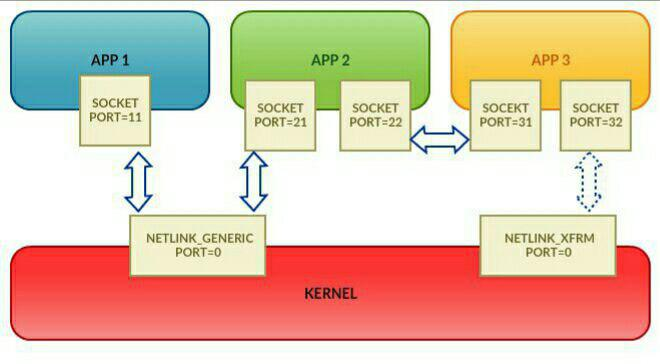
\includegraphics[width=15cm]{netlink_comunication}%inserisce una figura larga 5cm
                                        %se si vuole usare va scommentata
%
%%%%%%%%%%%%%%%%%%%%%%%%%%%%%%%%%%%%%%%%%inserisce la legenda ed etichetta
                                        %   la figura con \label{fig:prima}
\caption[comunicazione netlink]{scambio di messaggi attraverso socket netlink}
\end{center}
\end{figure}\\
L'interfaccia di comunicazione \`e abbastanza standardizzata ma personalizzabile a livello di payload, ognuno pu\`o definire una struttura personalizzata per poi usarla per comunicare attraverso i socket netlink con altri processi.
\subsection{Libnl}
Netlink Protocol Library Suite (libnl), \`e una raccolta di librerie ed utility che forniscono API di comunicazione netlink basate su quelle del kernel linux e comprende \cite{K10}:
\begin{description}                     %crea un elenco descrittivo
  \item[libnl] Core della libreria, offre uno strato di unificazione delle interfacce sulle quali poi si basano le altre librerie che pertanto di pendo da questa;
  \item[libnl-route] Questa libreria si occupa di fornire API per la configurazione degli elemnti della famiglia NETLINK\_ROUTE;
  \item[libnl-genl] genl significa generic netlink e questa libreria offre una versione estesa del protocollo netlink;
  \item[libnl-nf] API per configurazioni netlink basate su netfilter.

\end{description}
%%%%%%%%%%%%%%%%%%%%%%%%%%%%%%%%%%%%%%%%%non numera l'ultima pagina sinistra

\clearpage{\pagestyle{empty}\cleardoublepage}
